\documentclass{article}
\usepackage{graphicx,amssymb,amsmath,amsfonts,fancyhdr,wrapfig,refcount,amsthm}
\usepackage{times}
\usepackage{microtype}
\usepackage{subfigure}
\usepackage{latexsym}
\usepackage{bbm}
\usepackage{enumerate}
\usepackage{caption}
\usepackage{lineno}
\usepackage{xcolor}
\usepackage[pdfpagelabels,naturalnames,colorlinks]{hyperref}

\theoremstyle{plain}% default
\newtheorem{proposition}{Proposition}
\newtheorem{theorem}{Theorem}
\newtheorem{lemma}{Lemma}
%----- Macros and Definitions -----------------------------------
\newtheorem{observation}{Observation}

\hypersetup{colorlinks,breaklinks,
            urlcolor=[rgb]{.8,0.4,.8},
            linkcolor=[rgb]{0.2,0.2,.8},
            citecolor=[rgb]{.8,.2,.2}}

\newcommand{\NN}{\mathbb{N}} %  set of natural numbers
\newcommand{\ZZ}{\mathbb{Z}} %  set of integer number
\newcommand{\RR}{\mathbb{R}} %  set of real numbers
\newcommand{\SH}{\mathbb{S}} %  set of unit vectors
\newcommand{\HH}{{\cal H}} %  Calligraphic H
\newcommand{\PP}{{\cal P}} %  Calligraphic P
\newcommand{\DD}{{\cal D}} %  Calligraphic Q

\newcommand{\dist}{\operatorname{dist}}
\newcommand{\reals}{\mathbb{R}}

\def\etal{{et~al.}}
\def\ie{{i.e.}}
\def\eg{{e.g.}}
\def\slope{{\rm slope}}

\def \proof {\par \noindent {\bf Proof.}\hskip 5pt}
\def \endproof {\hfill $\Box$ \smallskip}

%---------------------- Title ---------------------------------------------

\title{Realization of simply connected polygonal linkages\\ and recognition of unit disk contact trees}
% \author{Clinton Bowen\inst{1}
% \and Stephane Durocher\inst{2}
% \and Maarten L\"offler\inst{3}
% \and Anika Rounds\inst{4}
% \and\\
%     Andr\'e Schulz\inst{5}
% \and Csaba~D.~T\'oth\inst{1,4}}

%\institute{Department of Mathematics, California State University Northridge, Los Angeles, CA, USA\\
%\email{clinton.bowen@my.csun.edu, csaba.toth@csun.edu}
%\and
%Department of Computer Science, University of Manitoba, Winnipeg, MB, Canada\\
% \email{durocher@cs.umanitoba.ca}
% \and
% Department of Information and Computing Sciences, Utrecht University, the Netherlands
% \email{m.loffler@uu.nl}
% \and
% Department of Computer Science, Tufts University, Medford, MA, USA
% \email{anika.rounds@tufts.edu, cdtoth@cs.tufts.edu}
% \and
% Theoretical Computer Science, University of Hagen, Hagen, Germany
% \email{andre.schulz@fernuni-hagen.de}
% }

% \authorrunning{Bowen, Durocher, L\"offler, Rounds, Schulz and T\'oth }% Part of LEFT running header
% \titlerunning{Realization of polygonal linkages and recognition of unit disk contact trees}

\begin{document}
\maketitle
\pagestyle{empty}
 
\begin{abstract}
We wish to decide whether a simply connected flexible polygonal structure can be realized in Euclidean space. Two models are considered: polygonal linkages (body-and-joint framework) and contact graphs of unit disks in the plane. (1) We show that it is strongly NP-hard to decide whether a given polygonal linkage is realizable in the plane when the bodies are convex polygons and their contact graph is a tree; the problem is weakly NP-hard already for a chain of rectangles, but efficiently decidable for a chain of triangles hinged at distinct vertices. (2) We also show that it is strongly NP-hard to decide whether a given tree is the contact graph of interior-disjoint unit disks in the plane.
\end{abstract}

\section{Introduction}\label{sec:intro}

In this paper, we study the realizability of complex structures that are specified by their local geometry.
The complex structures are represented as graphs with constraints on the separation between their vertices, and we ask if these graphs can be embedded in the plane subject to the constraints.
We consider two models in the plane; refer to Fig.~\ref{fig:1}.

\begin{enumerate}
\item A \textbf{polygonal linkage} is a set $\PP$ of convex polygons, and a set $H$ of hinges, where each hinge $h\in H$ corresponds to two or more points on the boundaries of distinct polygons in $\PP$. A \textbf{realization} of a polygonal linkage is an interior-disjoint placement of congruent copies of the polygons in $\PP$ such that the points corresponding to each hinge are identified. A \textbf{realization with orientation} uses only translated or rotated copies of the polygons in $\PP$ (no reflections) and for each hinge, the cyclic order of incident polygons is given. The topology of a polygonal linkage can be represented by the \textbf{hinge graph}, a bipartite graph where the vertices correspond to polygons in $\PP$ and the hinges in $H$, and edges represent the polygon-hinge incidences.
\item An (abstract) graph is a \textbf{coin graph} if it is the intersection graph of a set of interior-disjoint unit disks in the plane (where the vertices correspond to disks and two vertices are adjacent if and only if the corresponding disks are in contact). A \textbf{coin graph with embedding} is a coin graph \emph{together with} a cyclic order of the neighbors for each vertex (i.e., each disk).
\end{enumerate}

\begin{figure}[htbp]
  \centering
 \includegraphics[width=0.98\textwidth]{fig1+}
\caption{(a) A set of convex polygons and hinges.
(b) A realization of the polygonal linkage (with fixed orientation).
(c) A graph $G$ with 8 vertices.
(d) An arrangement of interior-disjoint unit disks whose contact graph is $G$.}
\label{fig:1}
\end{figure}

The {\sc Polygonal Linkage Realizability (PLR)} problem asks whether a given polygonal linkage admits a realization; and {\sc PLR with fixed orientation} asks whether it admits a realization with a given orientation. The {\sc Coin Graph Recognition (CGR)} problem asks whether a given (abstract) graph $G$ is the contact graph of interior-disjoint unit disks in the plane; and {\sc CGR with fixed embedding} asks whether a given plane graph $G$ is the contact graph of interior-disjoint unit disks in the plane with the same counterclockwise order of neighbors at each vertex.

These problems, in general, are known to be NP-hard (see details below). However, the hardness reductions crucially rely on graphs with a large number of cycles. We revisit these problems for simply connected topologies, where the hinge graph and the coin graph are trees.

\paragraph{Summary of results.}
Our main result is that the realizability problem remains NP-hard for simply connected polygonal linkages, the only exceptions are chains of triangles or rectangles hinged at distinct vertices. In an attempt to identify the most general problem that is not NP-hard, we considered several variants. Some variants are always realizable, some have easy hardness reductions, and some reductions required substantial new machinery. Our most demanding result is the NP-hardness of the recognition of \emph{coin trees} with fixed embedding. We summarize the results here.

\begin{enumerate}
\item We start with \emph{chains of polygons}, that is, polygonal linkages in which the hinge graph is a path (Section~\ref{sec:path}). It is easy to see that every chain of triangles or rectangles hinged together at distinct vertices is realizable and a realization can be computed efficiently. However, the problem becomes weakly NP-hard for chains of convex quadrilaterals hinged at distinct vertices or for  chains of triangles where one hinge may be at anywhere on the boundary. Our reduction uses {\sc Partition}.
\item We show that {\sc PLR} (with arbitrary orientation) is strongly NP-hard when the hinge graph is a tree, using an easy reduction from {\sc 3SAT} with the classic logic engine method (the proof is available in the full paper). The reduction crucially depends on possible reflections of the polygons.
\item We show that {\sc PLR} with fixed orientation is also strongly NP-hard when the hinge graph is a tree (Section~\ref{sec:hinge}), using a significantly more involved reduction from {\sc Planar3SAT}. We carefully design gadgets for variables, clauses and a planar graph to simulate {\sc Planar3SAT}.
\item We reduce the recognition of coin trees with fixed embedding to the previous problem ({\sc PLR} with fixed orientation), by simulating suitable polygons with an arrangement of unit disks (Section~\ref{sec:disk}). It would be easy to model a polygon by a \emph{rigid} coin graph (e.g., a section of the triangular grid), but all rigid graphs induce cycles. The main technical difficulty is that when the coin graph is a tree, any realization with unit disks is highly flexible, and simulating a rigid object becomes a challenge. We construct coin trees with ``stable'' realizations, which may be of independent interest.
\end{enumerate}

\paragraph{Related Previous Work.}
Previous research has established NP-hardness in several easy cases, but realizability for simply connected structures remained open. Polygonal linkages (or body-and-joint frameworks) are a generalization of classical linkages (bar-and-joint frameworks) in rigidity theory. A linkage is a graph $G=(V,E)$ with given edge lengths. A realization of a linkage is a (crossing-free) straight-line embedding of $G$ in the plane. Based on ideas developed by Bhatt and Cosmadakis~\cite{BC87}, who proved that the realizability of linkages is NP-complete on the integer grid, the \emph{logic engine} method~\cite{BET+99,EW96,FHW97,HK01} has become a standard tool for proving NP-hardness in graph drawing. The logic engine is a graph composed of rigid 2-connected components, where two possible realizations of a 2-connected component encode a binary variable.

However, the logic engine method is \textbf{not} applicable to problems with fixed embedding or orientation, where the circular order of the neighbors of each vertex is part of the input. Cabello et al.~\cite{CDR07,EW90} used a significantly more elaborate reduction to show that the realizability of 3-connected linkages (where the orientation is unique by Whitney's theorem~\cite{W33}) is NP-hard. This problem is efficiently decidable, though, for near-triangulations~\cite{CDR07,BV96}.

Note that every \emph{tree} linkage can be realized in $\RR^2$ with almost collinear edges. According to the celebrated \emph{Carpenter's Rule Theorem}~\cite{CDR03,Str05}, every realization of a path (or a cycle) linkage can be continuously moved (without self-intersection) to any other realization. In other words, the realization space of such a linkage is always connected. However, there are trees of maximum degree 3 with as few as 8 edges whose realization space is disconnected~\cite{BCD+09}; and deciding whether the realization space of a tree linkage is connected is PSPACE-complete~\cite{AKR+04}.
(Earlier, Reif~\cite{Rei79} showed that it is PSPACE-complete to decide whether a polygonal linkage can be moved from one realization to another among polygonal obstacles in $\RR^3$.)
Cheong et al.~\cite{CdG+07} consider the ``inverse'' problems of introducing the minimum number of point obstacles to reduce the configuration space of a polygonal linkage to a unique realization.

Connelly et al.~\cite{CDD+10} showed that the Carpenter's Rule Theorem generalizes to certain polygonal linkages obtained by replacing the edges of a path linkage with special polygons (called \emph{slender adornments}). Our Theorem~\ref{thm:hinge2} indicates that if we are allowed to replace the edges of a linkage with arbitrary convex polygons, then deciding whether the realization space is empty or not is already NP-hard.

Recognition problems for intersection graphs of various geometric object have a rich history~\cite{HK01}. Breu and Kirkpatrick~\cite{BK98} proved that it is NP-hard to decide whether a graph $G$ is the contact graph of unit disks in the plane, i.e., recognizing \emph{coin graphs} is NP-hard; see also~\cite{BET+99}. Recognizing outerplanar coin graphs is already NP-hard, but decidable in linear time for caterpillars~\cite{KNR15}. It is also NP-hard to recognize the contact graphs of pseudo-disks~\cite{HK01} and disks of bounded radii~\cite{BK95} in the plane, and unit disks in higher dimensions~\cite{Hli97,HK01}. All these hardness reductions produce graphs with a large number of cycles, and do not apply to trees. Note that the contact graphs of disks \emph{of arbitrary radii} are exactly the planar graphs (by Koebe's circle packing theorem), and planarity testing is polynomial. Consequently, every tree is the contact graph of disks of \emph{some} radii in the plane.
However, deciding whether a given star is realizable as a contact graph of disks of given radii but arbitrary embedding is already NP-hard~\cite{KNR15}.

Eades and Wormald~\cite{EW90} showed that it is NP-hard to decide whether a given tree is a \emph{subgraph} of a coin graph. Schaefer~\cite{Sch13} proved that deciding whether a graph with given edge lengths can be realized by a straight-line drawing (possibly with crossing edges) has the same complexity as the existential theory of the reals. Both reductions crucially rely on a large number of cycles. Our work is the first to simulate rigid polygons with truly flexible combinatorial structures that have simply connected topology.

\section{Chains of Polygons\label{sec:path}}

In this section, we consider polygonal linkages whose hinge graph is a path. We call such a linkage a \emph{chain of polygons}, given by a sequence of convex polygons $(P_1,\ldots, P_n)$, and $n-1$ hinges, where the $i$th hinge corresponds to a pair of points on the boundaries of $P_i$ and $P_{i+1}$, for $i=1,\ldots, n-1$.
Generalizing an observation by Demaine et al.~\cite{DEEH02}[Lemma~2], we formulate a simple sufficient condition for the realizability of a chain of polygons.

\begin{proposition}\label{pp:chain}
Consider a chain of convex polygons $(P_1,\ldots , P_n)$ with $n-1$ hinges.
If $P_i$ admits parallel tangent lines through both of its hinges for $i=2,\ldots ,n-1$,
then the chain of polygons is realizable with fixed orientation. Furthermore, a
realization can be computed in $O(n)$ time.
\end{proposition}
It follows that every chain of triangles (resp., rectangles) hinged at distinct vertices is realizable with fixed orientation.
Surprisingly, the realizability of a chain of arbitrary polygons is already NP-hard, even if the polygons are convex quadrilaterals hinged at vertices, or triangles hinged at arbitrary boundary points. We reduce the problem from {\sc Partition}, which is weakly NP-hard (i.e., NP-hard when the input is a sequence of $n$ integers between 1 and $2^n$). We give two NP-hardness proofs for the problem: an easier reduction for the case where reflections of polygons are allowed, and, as an extension,  a more technical proof for the case when the orientation of the polygons is fixed. The main idea behind both proofs is that any realization of the chain enforces a bounded rectangular region (frame) in which the remaining polygons have to be fitted. The width of the remaining polygons encode the integers given by the {\sc Partition} instance. Simply speaking, the joint of the first and the last polygon inside the frame have to be vertically aligned to get the last big polygon in. This is possible if and only if we have a yes-instance for {\sc Partition}. See Fig.~\ref{fig:chain} for an example of the reduction, further details are given in the full paper.

\begin{figure}[htbp]
  \centering
 \includegraphics[width=0.95\textwidth]{fig-chains}
\caption{(a) A chain of 8 rectangles encode {\sc Partition} for 3 integers $(a_1,a_2,a_3)$.
Rectangles $f_1,\ldots, f_4$ form a frame around a rectangle $R$ in any realization.
(b) A chain of 16 polygons encode {\sc Partition} for 3 integers $(a_1,a_2,a_3)$.}
\label{fig:chain}
\end{figure}

For the second proof we first reduce to instances in which the chained polygons are either triangles, rectangles, or hexagons
that are formed by rectangles of height~2 from which an isosceles triangle of side lengths 1 is cut off on every corner.
We then replace these polygons by a subchain of triangles whose unique realization redefines these shapes (Fig.~\ref{fig:triangles} depicts this idea).
\begin{figure}[htbp]
  \centering
 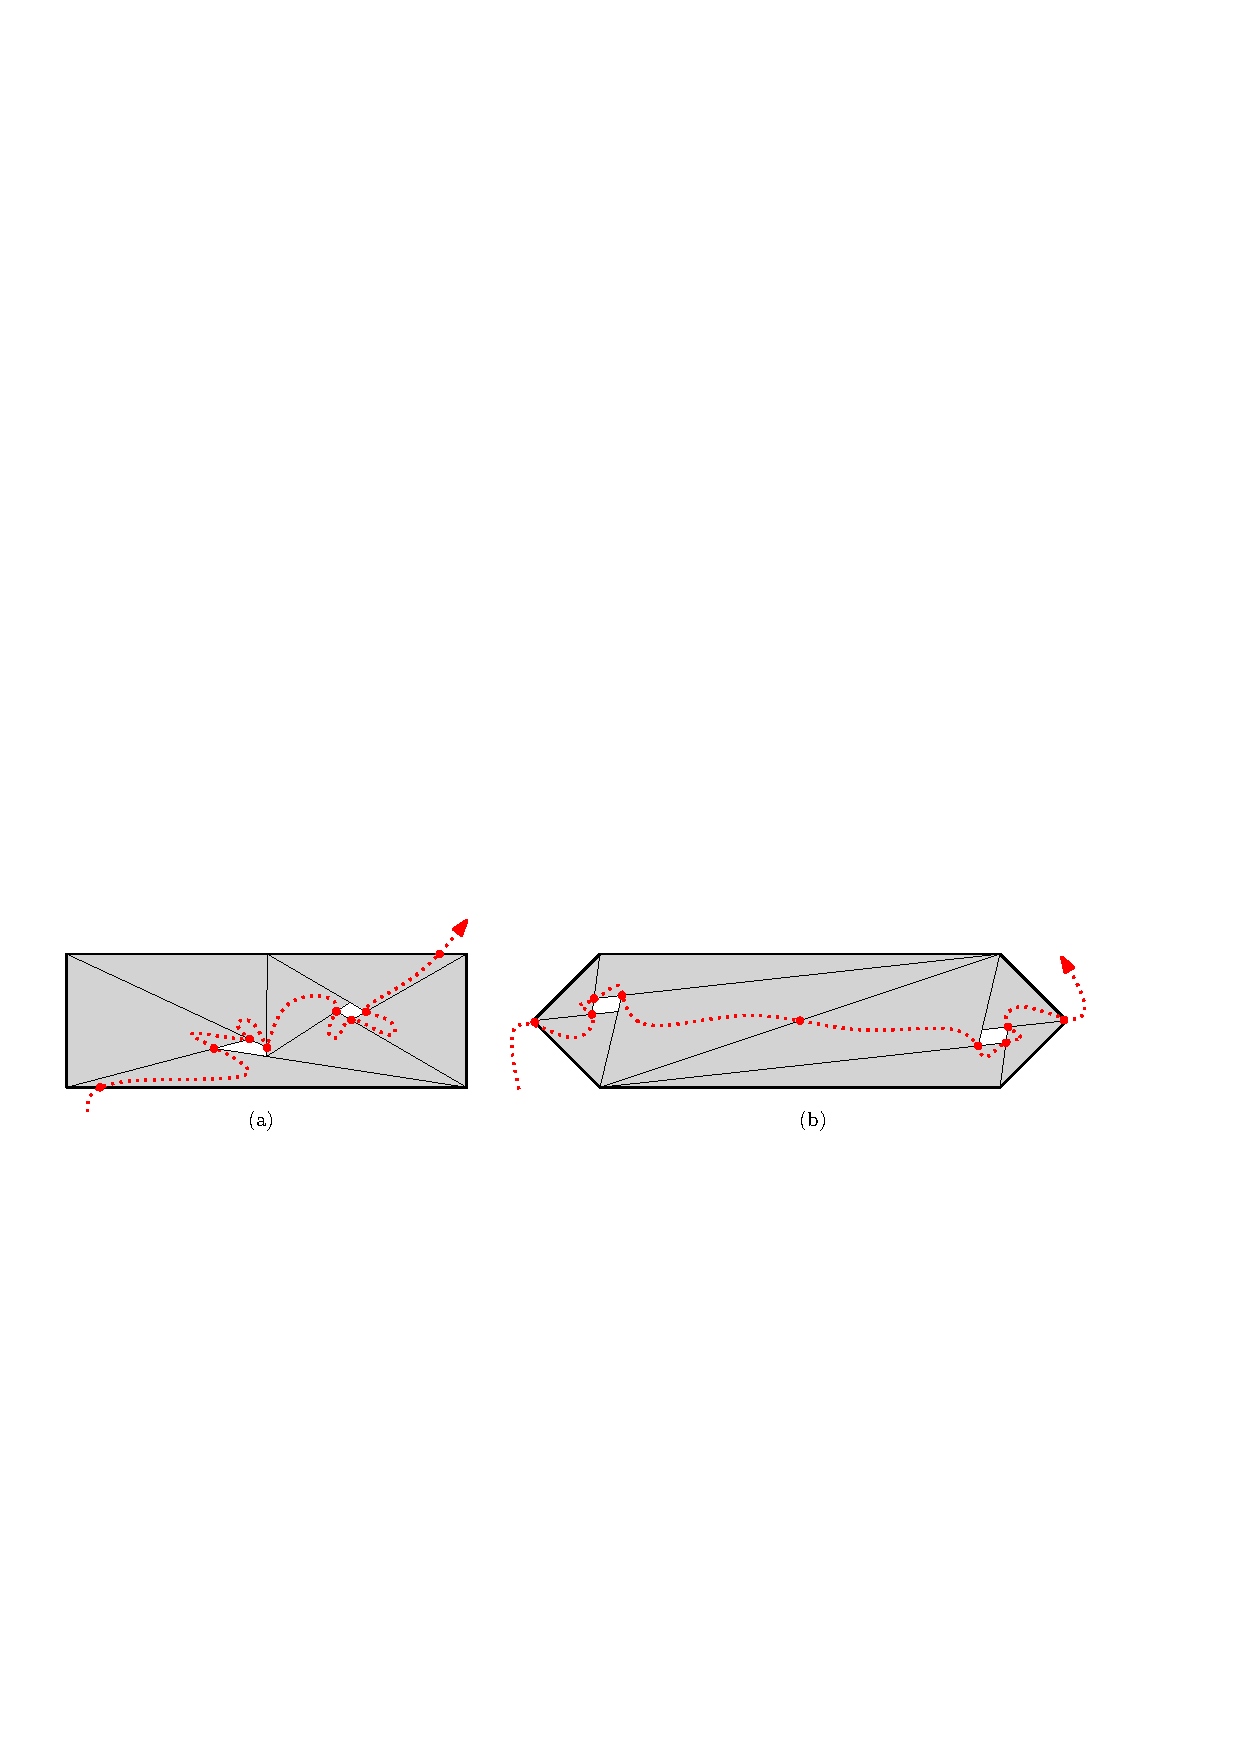
\includegraphics[width=0.8\textwidth]{fig-triangles}
\caption{(a) A rectangle with two hinges on opposite sides is split into a chain of 8 triangles, which has a unique realization (even with reflections).
(b) A hexagon with two hinges at opposite vertices is split into a chain of 8 triangles,
which has a unique realization with fixed orientation.}
\label{fig:triangles}
\end{figure}

\begin{theorem}\label{thm:path1}
It is weakly NP-hard to decide whether a chain of rectangles is realizable.
\end{theorem}

\begin{theorem}\label{thm:path2}
It is weakly NP-hard to decide whether a chain of convex polygons is realizable with fixed orientation. This is already true if the chain of polygons is formed by triangles whose hinges are not restricted to vertices.
\end{theorem}


\section{Realizability of Polygonal Linkages with Fixed Orientation\label{sec:hinge}}

\begin{theorem}\label{thm:hinge2}
It is strongly NP-hard to decide whether a polygonal linkage whose hinge graph is a \textbf{tree} can be realized with fixed orientation.
\end{theorem}

Our proof for Theorem~\ref{thm:hinge2} is a reduction from {\sc Planar-3-SAT} (P3SAT): decide whether a given Boolean formula in 3-CNF with a planar associated graph is satisfiable. The \emph{graph associated} to a Boolean formula in 3-CNF is a bipartite graph where the two vertex classes correspond to the variables and to the clauses, respectively; there is an edge between a variable $x$ and a clause $C$ iff $x$ or $\neg x$ appears in $C$. See Fig.~\ref{fig:assoc}(left).

\begin{figure}[htbp]
	\centering
	\includegraphics[width=0.7\columnwidth]{fig-assoc-hex}
	\caption[]{Left: the associated graph $A(\Phi)$ for a Boolean formula $\Phi$.
Right: the schematic layout of the variable, clause, and transmitter gadgets in our construction.}
	\label{fig:assoc}
\end{figure}

\paragraph{The big picture.}
Given an instance $\Phi$ of P3SAT with $n$ variables and $m$ clauses, we construct a simply connected polygonal linkage $(\PP,H)$, of polynomial size in $n$ and $m$, such that $\Phi$ is satisfiable iff $(\PP,H)$ admits a realization with fixed orientation. We construct a polygonal linkage  in two main steps: First, we construct an auxiliary structure where some of the polygons have fixed position in the plane (called \emph{obstacles}), while other polygons are flexible, and each flexible polygon is hinged to an obstacle. Second, we modify the auxiliary construction into a polygonal linkage by allowing the obstacles to move freely, and by adding new polygons and hinges as well as an exterior \emph{frame} that holds the obstacle polygons in place. All polygons in our constructions are regular hexagons or long and skinny rhombi because these are the polygons that we can ``simulate'' with coin graphs in Section~\ref{sec:disk}.

We start with embedding the graph $A(\Phi)$ associated to $\Phi$ into a hexagonal tiling, and then replace the vertices by variable and clause gadgets, and the edges by transmitter gadgets (to be described below). A variable gadget corresponds to a cycle in the hexagonal tiling, a clause gadget to single vertex incident to three hexagons, and a transmitted gadget to a path along a sequence of edges and vertices of the tiling. Refer to Fig.~\ref{fig:assoc}(right).

The main idea for the auxiliary construction is the following. We thicken the edges of the hexagonal tiling into \emph{corridors} of uniform width, and the vertices of the tiling into regular triangles, which form \emph{junctions} between three corridors. The boundaries of the corridors form regular hexagons, which will be the obstacle polygons in our auxiliary construction. In each corridor, we insert flexible hexagons, with one corner hinged to the boundary of the corridor. Each flexible hexagon has two possible realizations (say, \emph{left} and \emph{right}) that can encode a binary variable: all flexible polygons turn in the same direction along a cycle (clockwise or counterclockwise) with suitable spacing between the hexagons (Fig.~\ref{fig:variable}(a-b)) and with a small flexible polygon at each junction (Fig.~\ref{fig:variable}(c)). Similarly, the value of a binary variable is transmitted via a chain of corridors and junctions. A clause of $\Phi$ is simulated by a single junction (Fig.~\ref{fig:clause}), where a small flexible polygon ensures that hexagons from at most two adjacent corridors enter the junction (i.e., at most two literals are false).

\paragraph{Auxiliary Construction: flexible hexagons in a rigid frame.}
Let $\Phi$ be a Boolean formula in 3CNF with variables $x_1,\ldots , x_n$ and clauses $C_1,\ldots ,C_m$, and let $A(\Phi)$ be the associated planar graph. We modify $A(\Phi)$ to obtain a plane graph $\tilde{A}(\Phi)$ of maximum degree 3 as follows: Replace each \emph{variable} vertex $v$ by a cycle whose length equals the degree of $v$, and distribute the edges incident to $v$ among the vertices of the cycle.

Embed $\tilde{A}(\Phi)$ into the section of a hexagonal tiling (Fig.~\ref{fig:assoc}), contained in a regular hexagon of side length $N$, where $N$ is a polynomial of $n$ and $m$~\cite{BK+98}. Let $t=2N^3+1$ ($t$ will be the number of flexible hexagons in a corridor). Scale the grid such that the cells become regular hexagons of side length $(5t-1)/2+\sqrt{3}$, and then scale each cell independently from its center to a hexagon of side length $(5t-1)/2$. These large hexagons are considered fixed obstacles in our auxiliary construction. Between two adjacent obstacle hexagons, there is a $\frac{5t-1}{2}\times \sqrt{3}$ rectangle, which we call a \emph{corridor}. Three adjacent corridors meet at a regular triangle, which we call a \emph{junction}. We next describe variable, clause, and transmitter gadgets.

\begin{figure}[htbp]
	\centering
	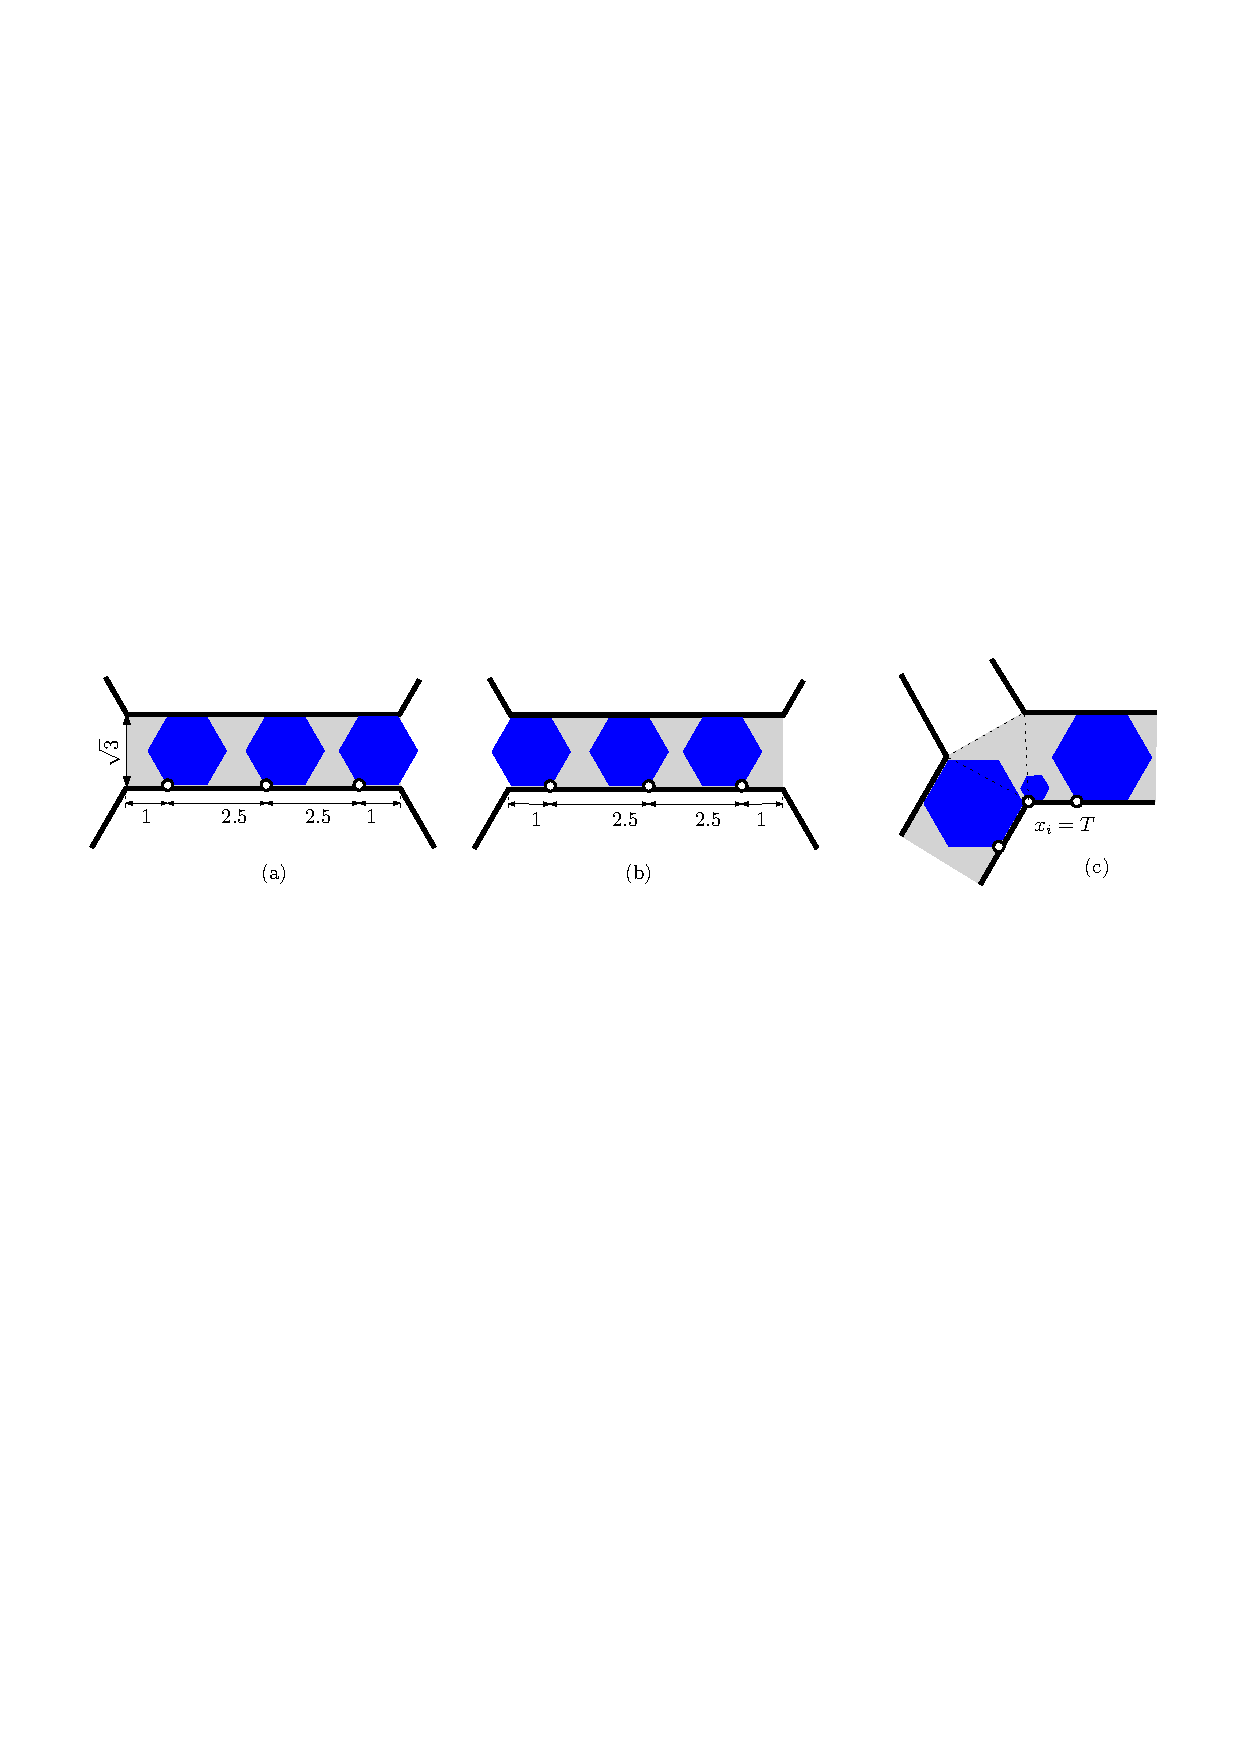
\includegraphics[width=0.9\columnwidth]{fig-variable-hex+}
	\caption{(a) A corridor when all unit hexagons are in state R.
(b) A corridor where all unit hexagons are in state L.
(c) A junction where a small hexagon between two corridors
    ensures that at most one unit hexagon enters the junction from those corridors.}
	\label{fig:variable}
\end{figure}

The basic building block of both variable and transmitter gadgets consists of $t$ regular hexagons of side length 1 (\emph{unit hexagons}, for short) attached to a wall of a corridor such that the hinges divide the wall into $t+1$ intervals of length $(1,2.5,\ldots ,2.5,1)$ as shown in Fig.~\ref{fig:variable}(a-b) for $t=3$. Since the height of the corridor is $\sqrt{3}$, each hexagon has exactly two possible realizations: it can lie either \emph{left} or \emph{right} of the hinge in a horizontal corridor. For simplicity, we use the same notation (R and L) in nonhorizontal corridors, too. Hence, the \emph{state} of each flexible hexagon in a realization is either L or R. The following observation describes the key mechanism of a corridor.

\begin{observation}\label{obs:corridor}
\begin{itemize}
\item[]
\item[(1)] If the leftmost hexagon is in state R, then all $t$ hexagons are in state R, and the rightmost hexagon enters the junction on the right of the corridor.
\item[(2)] Similarly, if the rightmost hexagon is in state L, then all $t$ hexagons are in state L, and the leftmost hexagon enters the junction on the left of the corridor.
\end{itemize}
\end{observation}

Each junction is a regular triangle, adjacent to three corridors. In some of the junctions, we attach a small hexagon of side length $\frac{1}{3}$ to one or two corners of the junction (see Fig.~\ref{fig:variable}(c) and Fig.~\ref{fig:transmitter}). Importantly, if such a small hexagon is attached to a vertex between two corridors, then a unit hexagon can enter the junction from at most one of those corridors.

The {\bf variable gadget} for variable $x_i$ is constructed as follows. Recall that variable $x_i$ corresponds to a cycle in the associated graph $\tilde{A}(\Phi)$, which has been embedded as a cycle in the hexagonal tiling, with corridors and junctions. In each junction along this cycle, attach a small hexagon in the common boundary of the two corridors in the cycle. Observation~\ref{obs:corridor} and the small hexagons ensure that the state of any unit hexagon along the cycle determines the state of all other unit hexagons in the cycle. This property defines the binary variable $x_i$: If $x_i=T$, then all unit hexagons in the top horizontal corridors are in state R; and if $x_i=F$, they are all in state L.

\begin{figure}[htbp]
	\centering
	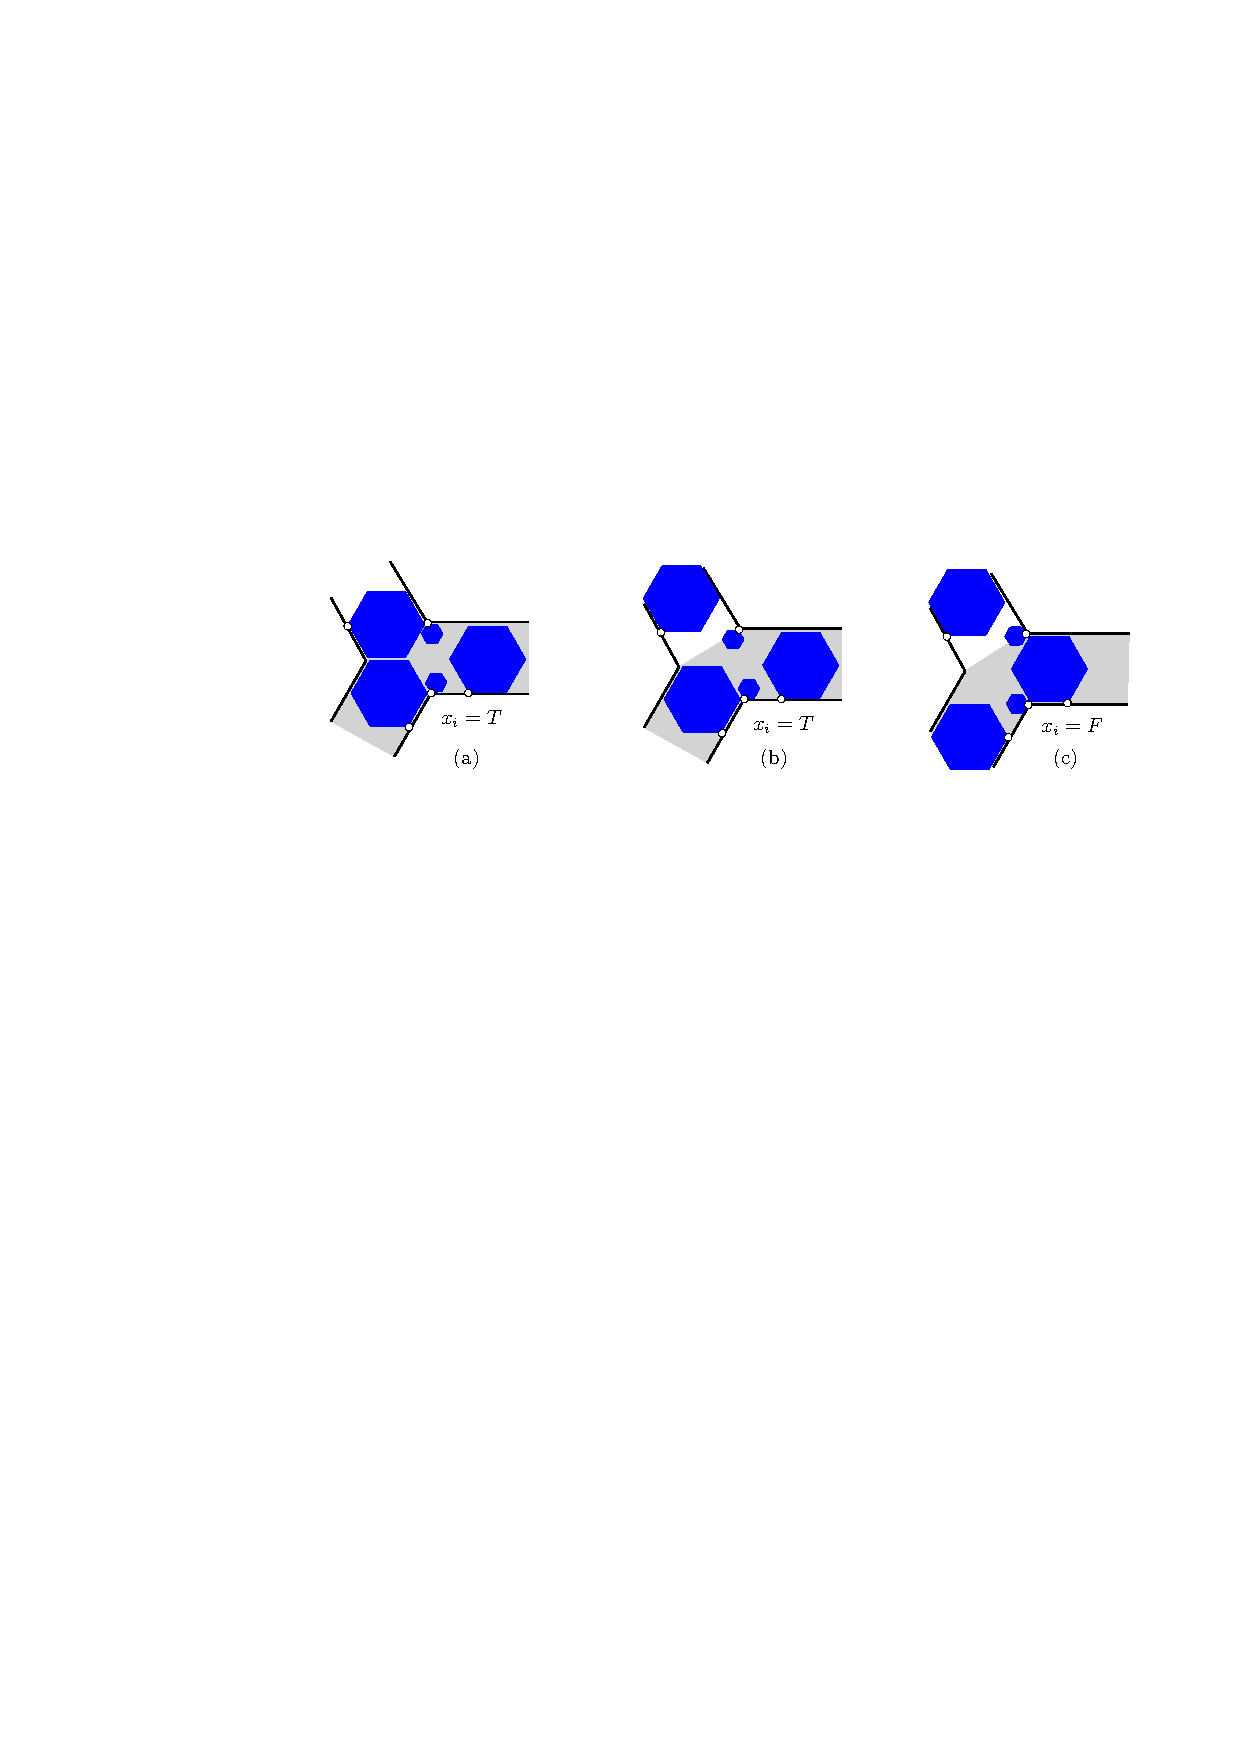
\includegraphics[width=0.7\columnwidth]{fig-transmitter-hex}
	\caption{The common junction of a variable gadget and a transmitter gadget.
(a) When $x_i=T$, a hexagon of the transmitter may enter the junction of the variable gadget.
(b) When $x_i=T$, the transmitter gadget has several possible realizations.
(c) When $x_i=F$, no hexagon from the transmitter enters a junction of the variable gadget.}
	\label{fig:transmitter}
\end{figure}

A {\bf transmitter gadget} is constructed for each edge $(x_i,C_j)$ of the graph $A(\Phi)$.
It connects a junction of the variable gadget $x_i$ with the junction representing the clause gadget $C_j$. The gadget consists of a path of corridors and junctions: at each interior junction, attach a small hexagon in the common boundary of the two corridors in the path (similarly to the variable gadget). At the common junction with the variable gadget $x_i$, we attach one additional small hexagon to one of the vertices (refer to Fig.~\ref{fig:transmitter}). If the literal $x_i$ (resp., $\overline{x}_i$) appears in $C_j$, then we attach a small hexagon to the corner of this junction such that if $x_i=F$ (resp., $\overline{x}_i=F)$, then the unit hexagon of the transmitter gadget cannot enter this junction. This ensures that false literals are always correctly transmitted to the clause junctions (and true literals can always transmit correctly).

The {\bf clause gadget} lies at a junction adjacent to three transmitter gadgets (see Fig.~\ref{fig:clause}). At such a junction, we attach a unit line segment to an arbitrary vertex of the junction, and a small hexagon of side length $\frac{1}{3}$ to the other end of the segment. If unit hexagons enter the junction from all three corridors (i.e., all three literals are false), then there is no space left for the small hexagon. But if at most two unit hexagons enter the junction (i.e., one of the literals is true), then the unit segment and the small hexagon are realizable.

\begin{figure}[htbp]
	\centering
	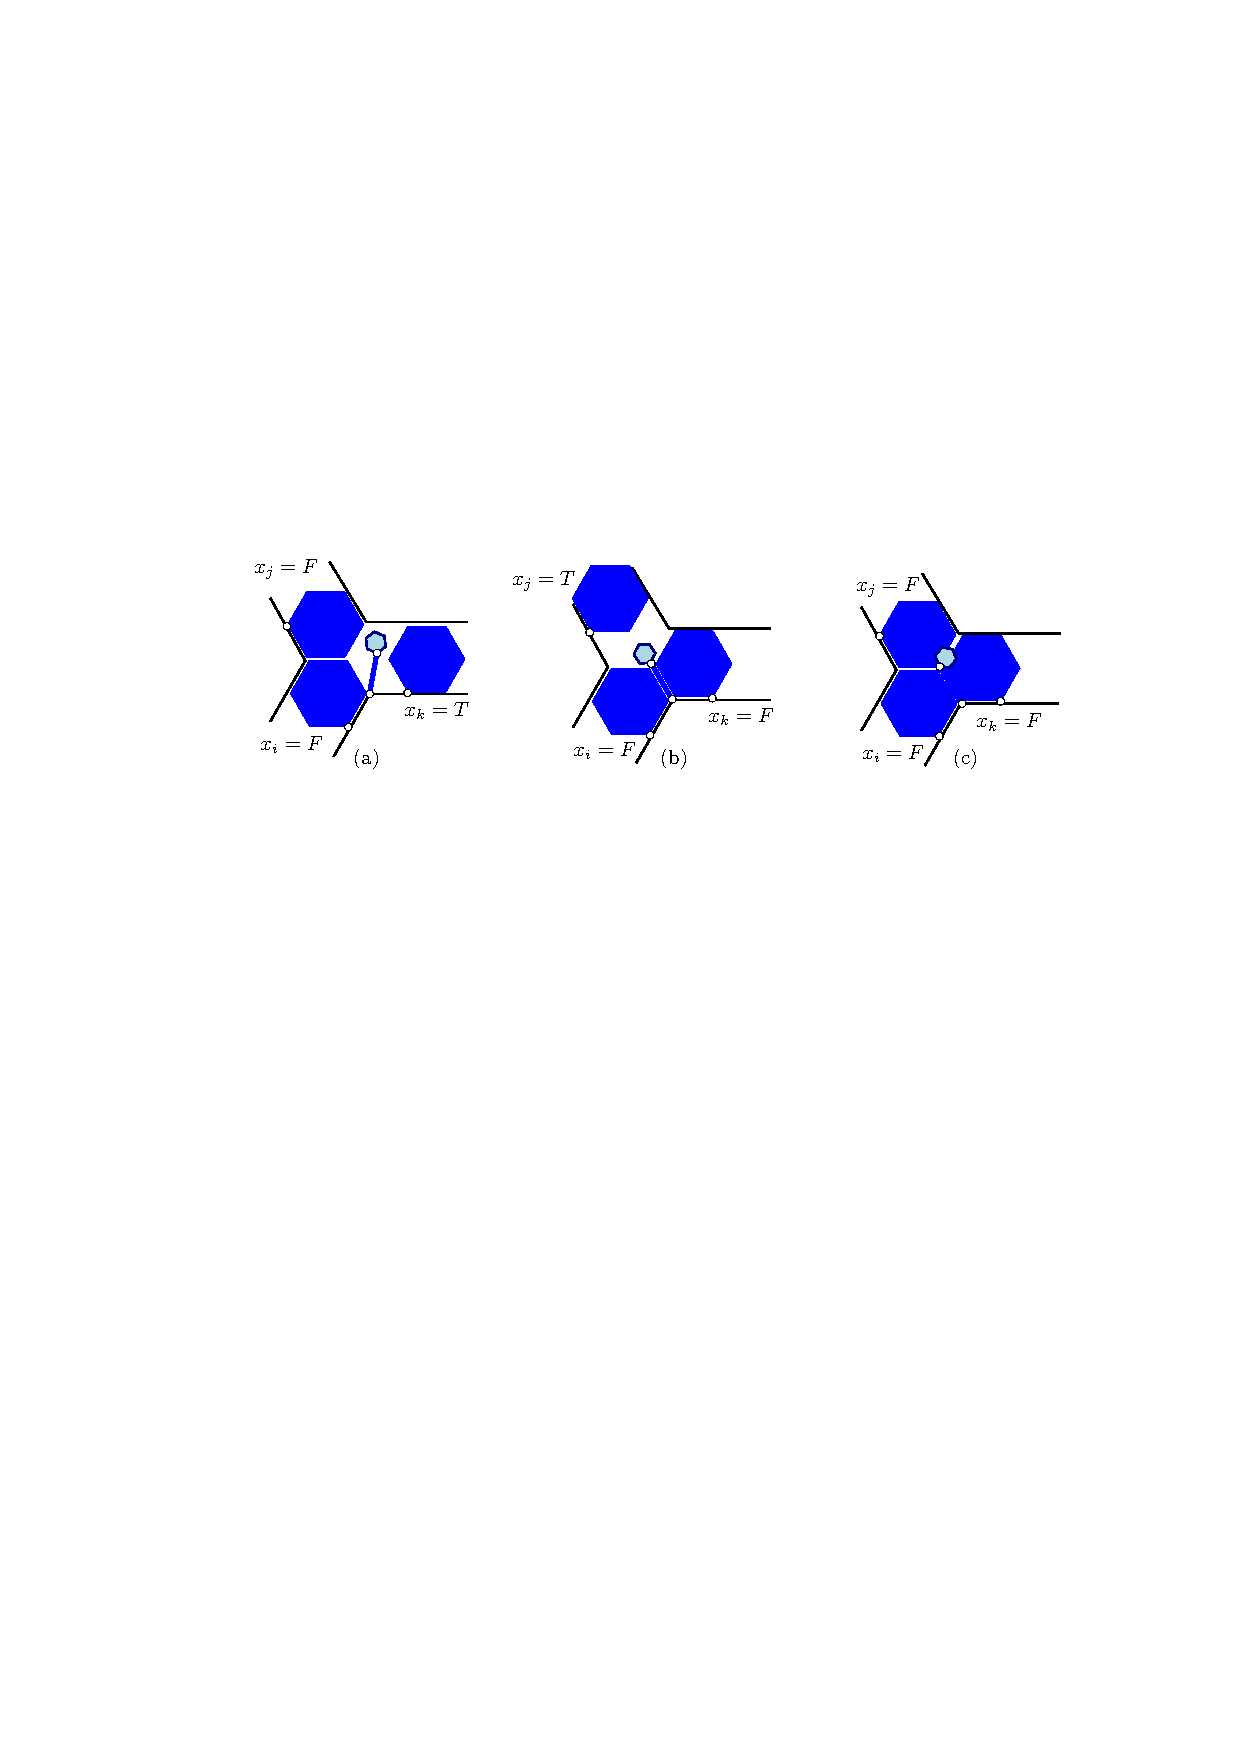
\includegraphics[width=0.7\columnwidth]{fig-clause-hex}
	\caption{(a-b) A clause gadget $(x_i\vee x_j\vee x_k)$ is
    realizable when at least one of the literals is {\sc True}.
    (c) The clause gadget cannot be realized when all three literals are {\sc False}.}
	\label{fig:clause}
\end{figure}

The following lemma summarizes our result about the auxiliary construction.
\begin{lemma}\label{lem:aux}
For every instance $\Phi$ of P3SAT, the above polygonal linkage with flexible and obstacle polygons
has the following properties: (1) it has polynomial size; (2) its hinge graph is a forest;
(3) it admits a realization such that the obstacle polygons remain fixed if and only if $\Phi$ is satisfiable.
\end{lemma}
The remaining details of our construction can be found in the full paper.

\section{Recognition of Coin Trees with Fixed Embedding\label{sec:disk}}

In this section, we reduce recognition of coin trees with fixed embedding from the realizability of polygonal linkages with cycle-free hinge graphs, which was shown to be strongly NP-hard in Section~\ref{sec:hinge}.

\begin{theorem}\label{thm:disk}
It is NP-hard to decide whether a given plane tree is a coin graph with fixed embedding.
\end{theorem}

It is enough to show that the polygons and the hinges used in Section~\ref{sec:hinge} can be simulated
by disks whose contact graphs are trees.
For a constant $\lambda>0$, we say that a coin graph $G$ with embedding is a \emph{$\lambda$-stable approximation} of a polygon $P$ if in every realization of $G$ as the contact graph of interior-disjoint unit disks, the Hausdorff distance between the union of disks and a congruent copy of $P$ is at most $\lambda$. In the remainder of this section,
 we design plane trees that approximate (i) a long and skinny rhombus, and (ii) a regular hexagon. We use these trees and suitable hinges to prove Theorem~\ref{thm:disk}.

Let $|ab|$ denote the Euclidean distance between points $a$ and $b$ in the plane,
and note that the distance between the centers of two kissing unit disks is precisely 2.
Let $\angle abc\in [0,2\pi)$ denote the counterclockwise angle that rotates
ray $\overrightarrow{ba}$ to $\overrightarrow{bc}$.
The following lemma about four unit disks is the key idea for our stability arguments.

\begin{lemma}\label{lem:P4lemma}
Let $(a,b,c,d)$ be a polygonal path in the plane such that $|ab|=|bc|=|cd|=2$
and the unit disks centered at $a$, $b$, $c$, and $d$ are interior-disjoint.
Then the sum of angles at the interior vertices on the left (resp., right)
of the chain is greater than $\pi$.
\end{lemma}
\begin{proof}
Without loss of generality, consider the two angles on the left
side at the two interior vertices, $\angle abc$ and $\angle bcd$.
We have $|ab|=|bc|=|cd|=2$, since the coin graph of the unit disks is $P_4$.
If $(a,b,c,d)$ is a rhombus, then $|ad|=2$ and $\angle abc+\angle bcd=\pi$.
Hence $|ad|>2$ implies $\angle abc+\angle bcd>\pi$.
\end{proof}

We construct a caterpillar graph on $n=8+4k$ vertices, for any $k \geq 0$,
and show that it is a 2-stable approximation of a long and skinny rectangle.
Recall that a \emph{caterpillar} is a tree in which all vertices are either on
or adjacent to a central path. For $k\geq 0$, let $T_k$ be a plane caterpillar
with central path $C=(a_{-k},\ldots, a_{-1},a_0,a_1,\ldots ,a_k)$ such that the
sequence of vertex degrees along the path is
\begin{equation}
1, \underbrace{3, \ldots, 3}_{k-2}, 4, 5, 4,
\underbrace{3, \ldots, 3}_{k-2}, 1 ,
\label{eq:caterpillarDegrees}
\end{equation}
and all leaves are attached to the left side of $C$.
Fig.~\ref{fig:tree}(left) shows that $T_k$ can be embedded as a subgraph
of a triangular grid. This embedding can be perturbed into a coin graph
(such that the distance between any two leaves is strictly more than 2).

\begin{lemma}\label{lem:stableTree}
For every integer $k\geq 0$, the plane tree $T_k$ in Fig.~\ref{fig:tree}~(left)
is a 2-stable approximation of a rhombus of width $2k+3$ and height $2+4\sqrt{3}$.
\end{lemma}

\begin{figure}
\centering
\includegraphics[width=.8\textwidth]{fig-ushape}
\caption{This caterpillar $T_6$ consists of two oppositely oriented chains,
each of which can only bend towards the other.}
\label{fig:tree}
\end{figure}

The proof of the lemma boils down to a careful estimation of the realizable distances
of the tree~$T_k$. With the help of Lemma~\ref{lem:P4lemma} we can show that
for every $j\ge 1$ the centers of $a_j$ and $a_{-j}$ lie at distance
at most 2 from their ``canonical'' position as indicated
in Fig.~\ref{fig:tree}(left). The proof goes via induction on~$j$ and
can be found in the full paper.

We can now extend the tree $T_k$ to a larger tree $T_k'$ with $\Theta(k^2)$ vertices as shown in Fig.~\ref{fig:hexagons}
that is a 2-stable approximation of a regular hexagon.
\begin{lemma}\label{lem:stablehex}
For every integer $k\geq 3$, the plane tree $T_k'$
is a 2-stable approximation of a regular hexagon of side length $2k$.
\end{lemma}
\begin{figure}
\centering
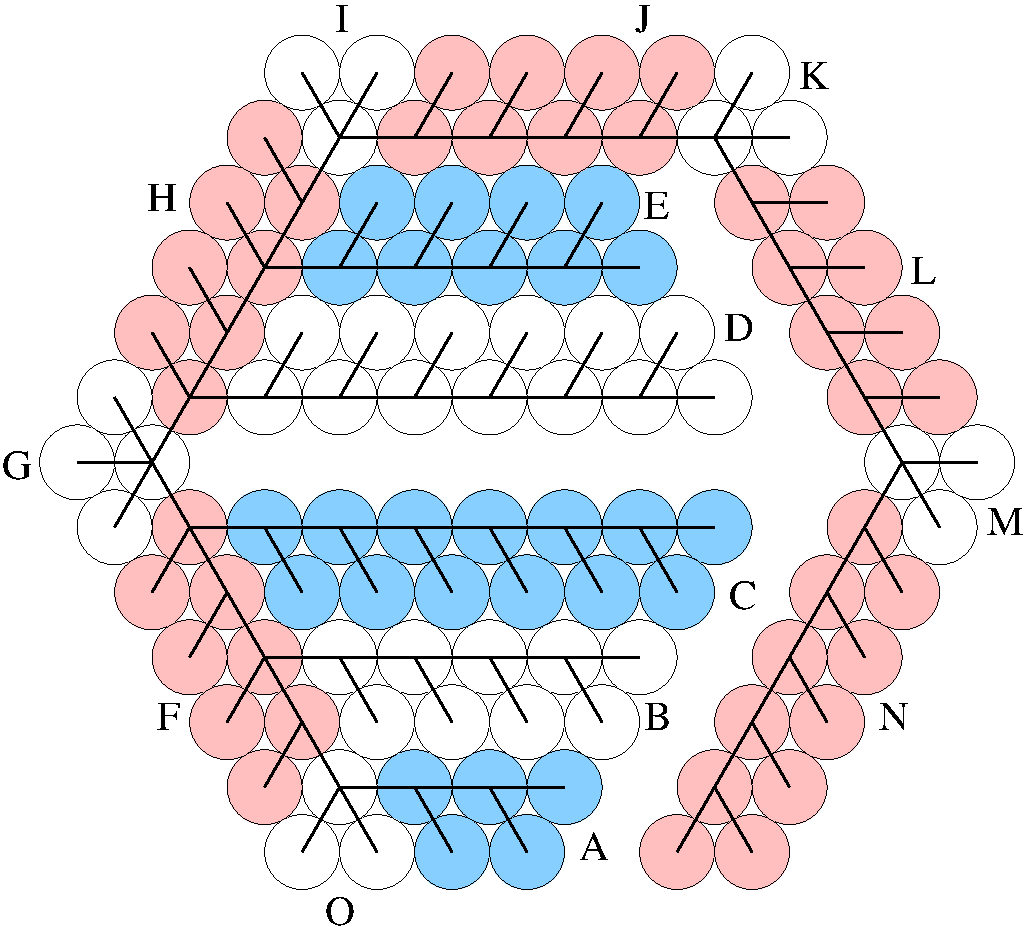
\includegraphics[width=.35\textwidth]{block3c}
\caption{The embedded tree $T_6'$ approximates a regular hexagon.}
\label{fig:hexagons}
\end{figure}
\begin{proof} (Sketch)
Let $k\geq 0$ be an arbitrary integer. To construct $T_k'$, consider five 3-regular
caterpillars, each of length $k$, joined in sequence at vertices of degree four
(except one joint vertex of degree five)
such that the leaf vertices lie on the outside. See Fig.~\ref{fig:hexagons}.
The joint vertices force five bends, each with a turn of more than $\pi/3$,
resulting in a hexagonal shape. The interior of the hexagon is filled
with pairs of 3-regular caterpillars aligned symmetrically across the
$x$-axis, similar to the realizations of $T_k$.
Since $T_k$ is a subgraph of $T_k'$,
the vertices in the subgraph are 2-stable
by Lemma~\ref{lem:stableTree} (c.f., the branches $C$ and $D$ in Fig.~\ref{fig:hexagons}).

By arguments analogous to those in the proof of Lemma~\ref{lem:stableTree},
additional horizontal branches are similarly constrained and, therefore,
also 2-stable (i.e., the branches $A$, $B$, $E$, and $J$ in Fig.~\ref{fig:hexagons}).
Similarly, the five branches forming the hexagon’s boundary (i.e., the branches $F$, $H$, $J$, $L$,
and $N$ in Fig.~\ref{fig:hexagons}) can only move towards the interior of the hexagon.
The empty space between any two disks is strictly less than one disk diameter,
and the result follows.
\end{proof}

We now have everything ready to give the reduction for Theorem~\ref{thm:disk}. Roughly speaking, we replace the polygons used in the reduction
that is presented in Sec.~\ref{sec:hinge} by stable approximations. The details of the proof of Theorem~\ref{thm:disk} are given in the full paper.

\section{Conclusions \label{sec:con}}

We have shown that deciding whether a simply connected polygonal linkage is realizable in the plane (with or without fixed orientation) is strongly NP-hard. The realizability of a chain of hinged polygons is weakly NP-hard (with or without fixed orientation); and it remains an open problem whether it is strongly NP-hard. 
 
Our hardness proof for the recognition of coin graphs with fixed embedding used subgraphs that ``approximate'' a regular hexagon. It remains an open problem whether a similar approximation is possible for coin graphs with \emph{arbitrary embedding}. We believe it is, but it would require an approximation of a ``dense'' packing of unit disks whose contact graph is a tree: this leads to a challenging problem in discrete geometry.

\paragraph{\bf Acknowledgements.} Our results in Section~\ref{sec:disk} were developed at the \emph{First International Workshop on Drawing Algorithms for Networks of Changing Entities (DANCE~2014)}, held in Langbroek, the Netherlands, and supported by the NWO project 639.023.208.
Research by Rounds and T\'oth was supported in part by the NSF awards CCF-1422311 and CCF-1423615.
Research by Durocher was supported in part by NSERC.

\begin{thebibliography}{99}

\bibitem{AKR+04}
H. Alt, C. Knauer, G. Rote, and S. Whitesides:
On the complexity of the linkage reconfiguration problem.
In: J. Pach (ed.) Towards a Theory of Geometric Graphs,
vol.~342 of Contemporary Mathematics, pp.~1--14,
AMS, Providence (2004), 

\bibitem{BCD+09}
B.~Ballinger, D.~Charlton, E.~D. Demaine, M.~L. Demaine, J.~Iacono, C.-H.~Liu, S.-H.~Poon:
Minimal locked trees.
In: F. Dehne, M.~Gavrilova, J-R. Sacks, and C.~D. T\'oth (eds.) WADS~2009, LNCS~5664, pp.~61-73, Springer, Heidelberg (2009)

\bibitem{BK+98}
T.~Biedl and G.~Kant:
A better heuristic for orthogonal graph drawings.
Comput. Geom. 9(3), 159--180 (1998).

\bibitem{BC87}
S.~N. Bhatt and S.~S. Cosmadakis:
The complexity of minimizing wire lengths in VLSI layouts.
Inform. Process. Lett. 25(4), 263--267 (1987)

\bibitem{BK95}
H. Breu and D.~G. Kirkpatrick:
On the complexity of recognizing intersection and touching graphs of discs.
In: F.~J. Brandenburd (ed.) GD 1995, LNCS~1027, pp.~88--98, Spinger, Heidelberg (1996)

\bibitem{BK98}
H.~Breu and D.~G. Kirkpatrick:
Unit disk graph recognition is NP-hard.
Comput. Geom. 9, 3--24 (1998)

\bibitem{CDR07}
S.~Cabello, E.~D.~Demaine, and G.~Rote:
Planar embeddings of graphs with specified edge lengths.
J.~Graph Alg. Appl.  11(1), 259--276 (2007)

\bibitem{CdG+07}
J.-S. Cheong, A.~F.~van der Stappen, K. Goldberg, M. H.~Overmars, and E.~Rimon:
Immobilizing hinged polygons.
Int. J. Comput. Geom. Appl. 17(1), 45--70 (2007).

\bibitem{CD-ch9}
R.~Connelly and E.~D. Demaine:
Geometry and topology of polygonal linkages.
In: J.~E. Goodman and J.~O'Rourke (eds.) \emph{Handbook of Discrete and Computational Geometry}, 
ch.~9, pp.~197--218, CRC, Boca Raton (2004)

\bibitem{CDR03}
R.~Connelly, E.~D.~Demaine, and G.~Rote:
Straightening polygonal arcs and convexifying polygonal cycles.
Discrete Comput. Geom. 30(2), 205--239 (2003).

\bibitem{CDD+10}
R.~Connelly, E.~D.~Demaine, M.~L.~Demaine, S.~P.~Fekete, S.~Langerman, J.~S.~B.~Mitchell, A.~Rib\'o, G.~Rote:
Locked and unlocked chains of planar shapes.
Discrete Comput. Geom. 44(2), 439--462 (2010)

\bibitem{DEEH02} 
E.~D. Demaine, D.~Eppstein, J.~Erickson, G.~W. Hart, and J.~O'Rourke:
Vertex-unfoldings of simplicial manifolds.
In 18th Sympos. on Comput. Geom., pp.~237--243, ACM Press, New York (2002)

\bibitem{BV96}
G.~Di~Battista and L.~Vismara:
Angles of planar triangular graphs.
SIAM J. Discrete Math. 9(3), 349--€“359 (1996)

\bibitem{BET+99}
G.~Di Battista, P. Eades, R. Tamassia, and I.~G. Tollis:
Graph Drawing: Algorithms for the Visualization of Graphs.
Prentice Hall, Upper Saddle River (1999)

\bibitem{EW96}
P.~Eades and S.~Whitesides:
The realization problem for Euclidean minimum spanning trees is NP-hard.
Algorithmica  16(1), 60--82 (1996)

\bibitem{EW90}
P.~Eades and N.~C.~Wormald: 
Fixed edge-length graph drawing is NP-hard.
Discrete Applied Mathematics 28, 111--134  (1990)

\bibitem{FHW97}
S.~P. Fekete, M.~E. Houle, and S.~Whitesides:
The wobbly logic engine: Proving hardness of non-rigid geometric graph representation problems.
In G.~Di~Battista (ed.) GD 1997, LNCS~1353, pp.~272--283, Springer, Heidelberg (1997)

\bibitem{Gre89}
A. Gregori:
Unit-length embedding of binary trees on a square grid.
Inform. Process. Lett. 31, 167--173 (1989)

\bibitem{Hli97}
P.~Hlin\v{e}n\'y:
Touching graphs of unit balls.
in G.~Di~Battista (ed.) GD 1997, LNCS~1353, pp.~350--358, Springer, Heidelberg (1997)

\bibitem{HK01}
P.~Hlin\v{e}n\'y and J.~Kratochv\'{\i}l:
Representing graphs by disks and balls (a survey of recognition-complexity results).
Discrete Mathematics 229(1-3), 101--124 (2001)

\bibitem{KNR15}
B.~Klemz, M.~N\"ollenburg and R.~Prutkin:
Recognizing weighted disk contact graphs.
In A. Lubiw and E. Di Giacomo (eds.) GD 2015, LNCS, Spinger, Heidelberg (2015)

\bibitem{Rei79} J.~H.~Reif:
Complexity of the mover's problem and generalizations.
In: 20th FoCS, pp.~421--427, IEEE, New York (1979)

\bibitem{Sch13}
M.~Schaefer: 
Realizability of graphs and linkages.
In J.~Pach (ed.) \emph{Thirty Essays on Geometric Graph Theory}, pp.~461--482, Springer, Heidelberg (2013)

\bibitem{Str05}
I.~Streinu:
Pseudo-triangulations, rigidity and motion planning.
Discrete Comput. Geom. 34(4), 587--635  (2005)

\bibitem{W33}
H.~Whitney:
Congruent graphs and the connectivity of graphs.
Amer. J. Math. 54, 150--168 (1932)

\end{thebibliography}

\end{document}

